\documentclass{article}
% translate with >> pdflatex -shell-escape <file>

% This file is an extract of the PGFPLOTS manual, copyright by Christian Feuersaenger.
% 
% Feel free to use it as long as you cite the pgfplots manual properly.
%
% See
%   http://pgfplots.sourceforge.net/pgfplots.pdf
% for the complete manual.
%
% Any required input files (for <plot table> or <plot file> or the table package) can be downloaded
% at
% http://www.ctan.org/tex-archive/graphics/pgf/contrib/pgfplots/doc/latex/
% and
% http://www.ctan.org/tex-archive/graphics/pgf/contrib/pgfplots/doc/latex/plotdata/

\usepackage{pgfplots}
\pgfplotsset{compat=newest}

\pagestyle{empty}

\begin{document}
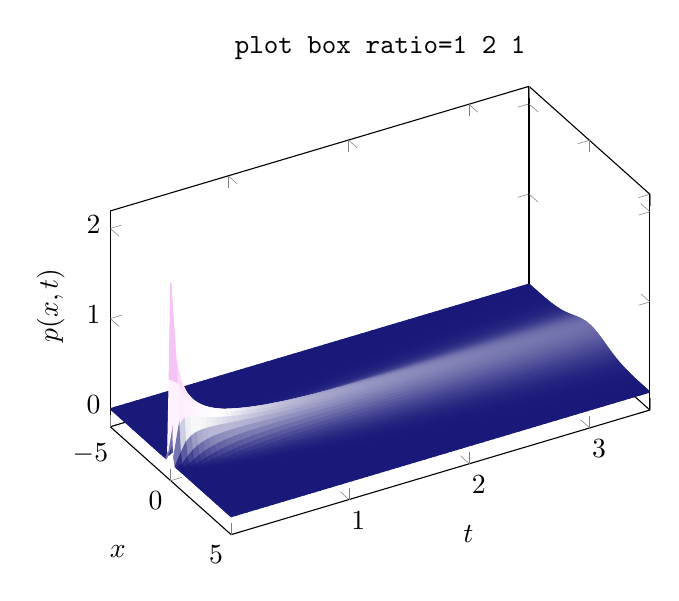
\begin{tikzpicture}
\begin{axis}[
	view/h=60,
	plot box ratio=1 2 1,
	colormap={violet}{[1cm] rgb255(0cm)=(25,25,122)
		color(1cm)=(white) rgb255(5cm)=(238,140,238)},
	xlabel=$x$,
	ylabel=$t$,
	zlabel={$p(x,t)$},
	shader=flat,
	title=\texttt{plot box ratio=1 2 1},
]
	\addplot3[surf,y domain=0.02:3.5,samples=81] 
		{1/(2*sqrt(pi*y)) * exp(0-x^2/y)};
	% the '0' is a work-around for a bug in PGF 2.00
\end{axis}
\end{tikzpicture}
\end{document}
